% Preambel
\documentclass[a4paper,openany]{report}


\usepackage{a4wide}
\usepackage[ansinew]{inputenc}
\usepackage[T1]{fontenc}
\RequirePackage{ifpdf}

\usepackage{hyperref}
	\hypersetup{%
  colorlinks=true,   % activates colored references
  pdfpagemode=None,  % PDF-Viewer starts without content et.al.
  pdfstartview=FitH, % PDF-Viewer uses a defined page width
  %linkbordercolor=111,
  % citebordercolor=111,
  citecolor=blue,
  linkcolor=blue}

\ifpdf
  \usepackage[pdftex]{graphicx}
	  \DeclareGraphicsExtensions{.pdf}
\else
  \usepackage[dvips]{graphicx}
	  \DeclareGraphicsExtensions{.eps}
\fi
	
\usepackage{fancyhdr}
\usepackage{booktabs}
%\usepackage[dvips]{rotating}
\usepackage{multirow}
\usepackage{multicol}

\usepackage{color}
\usepackage{amsmath}
\usepackage{alltt}
%\usepackage{array}
%\usepackage{colortbl}

\clubpenalty = 10000
\widowpenalty = 10000 \displaywidowpenalty = 10000

\definecolor{hellgrau}{gray}{0.95}
\definecolor{dunkelgrau}{gray}{0.55}



\renewcommand{\headrulewidth}{0pt} % no head rule
\renewcommand{\footrulewidth}{0pt} % no foot rule




%\nointend
%%%%%%%%%%%%%%%%%%%%%%%%%%%%%%
% start text here!!



\begin{document}
\pagenumbering{roman}

\title{A neural network toolbox for Octave\\
			Developer's Guide\\
			  Version: 0.1.9.1}

\author{M. Schmid}
\maketitle


\tableofcontents
\pagenumbering{arabic}

\chapter{Introduction}
This documentation isn't a well defined and structured docu for the neural network toolbox.
It's more a \textit{collection of my ideas and minds}.


\section{Installed system}
I'm developing and testing the actual version of the neural network toolbox on following 
program versions:

\begin{itemize}
  \item Octave 2.9.5
  \item octave-forge-2006.01.28
  \item OctPlot svn version
\end{itemize}

.. and on another system

\begin{itemize}
  \item Octave 2.9.12
  \item octave-forge packages ...
  \item OctPlot svn version
\end{itemize}


\section{Version numbers}

The first number describes the major release. Version number V1.0 will be the first toolbox release which should have the same functions like the Matlab R14 SP3 neural network Toolbox.\\

The second number defines the finished functions. So to start, only the MLPs will realised and so this will be the number V0.1.0.\\

The third number defines the status of the actual development and function. V0.1.0 means a first release with MLP. Actually it works only with Levenberg-Marquardt algorithm and Mean-Square-Error as performance function.
\section{Code convention}

The main function of this toolbox will be programed with help of the book in \cite{4}.
So the variables will have the same names like in the book with one exception: Variables, only with one letter, will have two letters, e.g. 
\begin{itemize}
	\item $X \rightarrow Xx$
	\item $Q \rightarrow Qq$
	\item $a \rightarrow aa$
\end{itemize}
and so on ...\\

This is only to make it possible to search for variable names.



\chapter{Octave's available functions}

\section{Available functions}
\subsection{min\_max}
\textit{min\_max} get the minimal and maximal values of an training input matrix. So the dimension of this matrix must be an RxN matrix where R is the number of input neurons and N depends on the number of training sets.\\

\noindent \textbf{\textcolor{brown}{Syntax:}}\\

\noindent mMinMaxElements = min\_max(RxN);\\

\noindent \textbf{\textcolor{brown}{Description:}}\\

\noindent RxN: R x N matrix of min and max values for R input elements with N columns\\ 

\noindent \textbf{\textcolor{brown}{Example:}}\\

\begin{equation}
	\left[
		\begin{array}{cc}
     	1 &  11 \\
    	0  & 21
   \end{array} 
	 \right]            = min\_max\left[ 
	 															   \begin{array}{ccccc}
	 															   3 & 1 & 3 & 5 & 11 \\
	 															   12& 0 & 21& 8 & 6  \\
	 															   \end{array}
	 															   	 \right]
\end{equation}


\chapter{Coding Guideline}
Some genereal descriptions why a variable has a chosen name. This is valid for the complete
toolbox... or so :-)\\
Here is only the description of variable names, which aren't visible to the user. Visible names are
described in the User's Guide!\\
The variable identifiers are taken from \cite{4}. One difference is purposeful added. If a variable has only one letter, a second small letter will be added to make it searchable. Who has ever tried to search a variable called "t"?

\section{Variable identifier}

\begin{tabbing}
\hspace*{1em} \= \textcolor{blue}{Identifier} \hspace*{3em}\= \textcolor{blue}{Description:} \\ 
  \textbf{Aa} \> \> hold the network values after transfer function.\\
  blf \>  \> \textbf{b}atch \textbf{l}earning \textbf{f}unction \\
  btf  \>  \> \textbf{b}atch \textbf{t}rainings \textbf{f}unction \\
  \textbf{Jj} \>  \> Jacobi matrix \\
  \textbf{Nn}  \> \> hold the network values before transfer function.\\  						
  net	\> \> structure which holds the neural network informations \\
  pf \>  \> \textbf{p}erformance \textbf{f}unction \\
  \textbf{Pp}				\>						\>input matrix; nInputs x nDataSets  \\
  \textbf{Pr}	\>		\> input range, this is a Nx2 matrix, that's why the capitalized P \\
  trf \>  \> \textbf{tr}ansfer \textbf{f}unction \\
  \textbf{Tt} \>  \> target matrix, nTargets x nDataSets\\
  \textbf{ss}	\> \> row vector with numbers of neurons in the layers, for each layer, one entry \\
  \textbf{vE}	\> \> row vector with errors... size depends on network structure. \\
  VV \>  \> Validation structure \\
  \textbf{xx} \>  \> Weight vector in column format\\
  
\end{tabbing}

\subsection{Nn}
\textbf{Nn} is a cell array and has one entry for each layer. In reality, this will have 2 or 3 layers.\\
In \textbf{Nn\{1,1\}} are the values for the first hidden layer. The size of this matrix depends
on the number of neurons used for this layer.\\
In \textbf{Nn\{2,1\}} are the values for the second hidden layer or the output layer. The size of this matrix depends
on the number of neurons used for this layer and so on ...\\
\textbf{Nn\{x,1\}} where \textbf{x} can be $\infty$.\\

\subsection{Aa}
\textbf{Aa} is a cell array and has one entry for each layer.\\
In \textbf{Aa\{1,1\}} are the values for the first hidden layer. The size of this matrix depends
on the number of neurons used for this layer.\\
In \textbf{Aa\{2,1\}} are the values for the second hidden layer or the output layer. The size of this matrix depends
on the number of neurons used for this layer.\\
See \textbf{Nn} for a more detailed description.\\

\subsection{vE}
\textbf{vE} is also a cell array which holds in the last (second) element the error vector. It's not completly clear, why in the last (second) element.\\
The number of rows depends on the number of output neurons. For one output neuron, \textbf{vE} holds only one row, for 2 output neurons, this holds of course 2 rows, and so on. 

\subsection{Jj}
This is the short term for the Jacobi matrix.
\chapter{Algorithm}
Here are some general thoughts about calculating parts are used in algorithm.

\section{Levenberg Marquardt}
This algorithm will be programed with \cite{4}.

\subsection{Sensitivity Matrix}
How does this looks like?\\
\begin{enumerate}
	\item for a 1-1-1 MLP
	\item for a 2-1-1 MLP
	\item for a 1-2-1 MLP
\end{enumerate}

\subsubsection{1-1-1 MLP}
In this case, the MLP holds one input neuron, one hidden neuron and one output neuron. The number of weights needed for this MLP is 4 (2 weights, 2 biases).\\

It needs two sensitivity matrices because the two layers. Each sensitivity matrix will hold 1 element.
This is taken from \cite{4}, example P12.5 page 12-44. Attention, in this example are two data sets used, this is the reason for the 4 elements...!

\subsubsection{2-1-1 MLP}
In this case, the MLP holds two input neurons, one hidden neuron and one output neuron. The number of weights needed for this MLP is 5 (3 weights, 2 biases).\\

It needs also two sensitivity matrices because the two layers. Actually, the input is not only a scalar, it is a vector with 2 elements. Even though, again after \cite{4}. I think the sensitivity matrices will hold only 1 element. So the number of elements will bi proportional to the number of hidden neurons and the number of output neurons.

\subsubsection{1-2-1 MLP}
In this case, the MLP holds one input neuron, two hidden neurons and one output neuron. The number of weights needed for this MLP is 7 (4 weights, 3 biases).\\

It needs also two sensitivity matrices because the two layers. Actually, the input is again only a scalar. 
Now calculating $n_1^1$ will result in a row vector with 2 elements. $n_1^2$ will hold only one element and so we have 3 elements in the sensitivity matrix.\\

We can say, the number of hidden neurons is responsible for the dimension of the sensitivity matrices.
For example, a 4-3-1 MLP with 100 data sets will generate following sensitivity matrix for the first layer:
$\tilde{\textbf{S}}^1 = [\tilde{\textbf{S}}^1_1 | \tilde{\textbf{S}}^1_2 | ... | \tilde{\textbf{S}}^1_{100}]$\\
\noindent $\tilde{\textbf{S}}^1_1$ will hold 3 elements  $\tilde{\textbf{S}}^1_1 = [\tilde{\textbf{S}}^1_{1,1} ~ \tilde{\textbf{S}}^1_{2,1} ~ \tilde{\textbf{S}}^1_{3,1}]^T$;
$\tilde{\textbf{S}}^1_2 = [\tilde{\textbf{S}}^1_{1,2} ~ \tilde{\textbf{S}}^1_{2,2} ~ \tilde{\textbf{S}}^1_{3,2}]^T$ and so on. So matrix will have a size of 3x100 for $\tilde{\textbf{S}}^1_{1}$
and a size of 1x100 for $\tilde{\textbf{S}}^1_{2}$.\\

By the way, the jacobian matrix will be a 100x20 matrix ..






\chapter{Function Index}

\section{Who calles who}
\begin{verbatim}
Function-File: isposint
=============================
\end{verbatim}
\begin{verbatim}
Function-File: logsig
=============================
\end{verbatim}
\begin{verbatim}
Function-File: min_max
=============================
\end{verbatim}
\begin{verbatim}
Function-File: newff
=============================
__init
__newnetwork
tansig
train
\end{verbatim}
\begin{verbatim}
Function-File: poststd
=============================
\end{verbatim}
\begin{verbatim}
Function-File: prestd
=============================
\end{verbatim}
\begin{verbatim}
Function-File: purelin
=============================
\end{verbatim}
\begin{verbatim}
Function-File: saveMLPStruct
=============================
__checknetstruct
__printAdaptFcn
__printAdaptParam
__printB
__printBiasConnect
__printBiases
__printIW
__printInitFcn
__printInitParam
__printInputConnect
__printInputWeights
__printInputs
__printLW
__printLayerConnect
__printLayerWeights
__printLayers
__printMLPHeader
__printNetworkType
__printNumInputDelays
__printNumInputs
__printNumLayerDelays
__printNumLayers
__printNumOutputs
__printNumTargets
__printOutputConnect
__printOutputs
__printPerformFcn
__printPerformParam
__printTargetConnect
__printTargets
__printTrainFcn
__printTrainParam
\end{verbatim}
\begin{verbatim}
Function-File: sim
=============================
__checknetstruct
logsig
purelin
tansig
\end{verbatim}
\begin{verbatim}
Function-File: subset
=============================
__optimizedatasets
\end{verbatim}
\begin{verbatim}
Function-File: tansig
=============================
\end{verbatim}
\begin{verbatim}
Function-File: train
=============================
__checknetstruct
__trainlm
\end{verbatim}
\begin{verbatim}
Function-File: trastd
=============================
\end{verbatim}
\begin{verbatim}
Function-File: __analyzerows
=============================
\end{verbatim}
\begin{verbatim}
Function-File: __calcjacobian
=============================
__dlogsig
__dpurelin
__dtansig
logsig
purelin
tansig
\end{verbatim}
\begin{verbatim}
Function-File: __calcperf
=============================
__mse
logsig
purelin
tansig
\end{verbatim}
\begin{verbatim}
Function-File: __checknetstruct
=============================
\end{verbatim}
\begin{verbatim}
Function-File: __copycoltopos1
=============================
\end{verbatim}
\begin{verbatim}
Function-File: __dlogsig
=============================
\end{verbatim}
\begin{verbatim}
Function-File: __dpurelin
=============================
\end{verbatim}
\begin{verbatim}
Function-File: __dtansig
=============================
\end{verbatim}
\begin{verbatim}
Function-File: __getx
=============================
__checknetstruct
\end{verbatim}
\begin{verbatim}
Function-File: __init
=============================
__checknetstruct
newff
\end{verbatim}
\begin{verbatim}
Function-File: __mae
=============================
\end{verbatim}
\begin{verbatim}
Function-File: __mse
=============================
\end{verbatim}
\begin{verbatim}
Function-File: __newnetwork
=============================
__checknetstruct
isposint
newff
train
\end{verbatim}
\begin{verbatim}
Function-File: __optimizedatasets
=============================
__analyzerows
__randomisecols
__rerangecolumns
\end{verbatim}
\begin{verbatim}
Function-File: __printAdaptFcn
=============================
\end{verbatim}
\begin{verbatim}
Function-File: __printAdaptParam
=============================
\end{verbatim}
\begin{verbatim}
Function-File: __printB
=============================
\end{verbatim}
\begin{verbatim}
Function-File: __printBiasConnect
=============================
\end{verbatim}
\begin{verbatim}
Function-File: __printBiases
=============================
\end{verbatim}
\begin{verbatim}
Function-File: __printInitFcn
=============================
\end{verbatim}
\begin{verbatim}
Function-File: __printInitParam
=============================
\end{verbatim}
\begin{verbatim}
Function-File: __printInputConnect
=============================
\end{verbatim}
\begin{verbatim}
Function-File: __printInputs
=============================
\end{verbatim}
\begin{verbatim}
Function-File: __printInputWeights
=============================
\end{verbatim}
\begin{verbatim}
Function-File: __printIW
=============================
\end{verbatim}
\begin{verbatim}
Function-File: __printLayerConnect
=============================
\end{verbatim}
\begin{verbatim}
Function-File: __printLayers
=============================
\end{verbatim}
\begin{verbatim}
Function-File: __printLayerWeights
=============================
\end{verbatim}
\begin{verbatim}
Function-File: __printLW
=============================
\end{verbatim}
\begin{verbatim}
Function-File: __printMLPHeader
=============================
\end{verbatim}
\begin{verbatim}
Function-File: __printNetworkType
=============================
newff
\end{verbatim}
\begin{verbatim}
Function-File: __printNumInputDelays
=============================
\end{verbatim}
\begin{verbatim}
Function-File: __printNumInputs
=============================
\end{verbatim}
\begin{verbatim}
Function-File: __printNumLayerDelays
=============================
\end{verbatim}
\begin{verbatim}
Function-File: __printNumLayers
=============================
\end{verbatim}
\begin{verbatim}
Function-File: __printNumOutputs
=============================
\end{verbatim}
\begin{verbatim}
Function-File: __printNumTargets
=============================
\end{verbatim}
\begin{verbatim}
Function-File: __printOutputConnect
=============================
\end{verbatim}
\begin{verbatim}
Function-File: __printOutputs
=============================
\end{verbatim}
\begin{verbatim}
Function-File: __printPerformFcn
=============================
\end{verbatim}
\begin{verbatim}
Function-File: __printPerformParam
=============================
\end{verbatim}
\begin{verbatim}
Function-File: __printTargetConnect
=============================
\end{verbatim}
\begin{verbatim}
Function-File: __printTargets
=============================
\end{verbatim}
\begin{verbatim}
Function-File: __printTrainFcn
=============================
train
\end{verbatim}
\begin{verbatim}
Function-File: __printTrainParam
=============================
train
\end{verbatim}
\begin{verbatim}
Function-File: __randomisecols
=============================
\end{verbatim}
\begin{verbatim}
Function-File: __rerangecolumns
=============================
__copycoltopos1
\end{verbatim}
\begin{verbatim}
Function-File: __setx
=============================
__checknetstruct
\end{verbatim}
\begin{verbatim}
Function-File: __trainlm
=============================
__calcjacobian
__calcperf
__getx
__setx
isposint
\end{verbatim}



\chapter{Test}

\section{isposint}
\begin{verbatim}
%!shared
%! disp("testing isposint")
%!assert(isposint(1)) # this should pass
%!assert(isposint(0.5),0) # should return zero
%!assert(isposint(-1),0) # should return zero
%!assert(isposint(-1.5),0) # should return zero
%!assert(isposint(0),0) # should return zero
%!fail("isposint([0 0])","Input argument must not be a vector, only scalars are allowed!")
%!fail("isposint('testString')","Input argument must not be a vector, only scalars are allowed!")
\end{verbatim}

\section{min\_max}
\subsection{min\_max}
\textit{min\_max} get the minimal and maximal values of an training input matrix. So the dimension of this matrix must be an RxN matrix where R is the number of input neurons and N depends on the number of training sets.\\

\noindent \textbf{\textcolor{brown}{Syntax:}}\\

\noindent mMinMaxElements = min\_max(RxN);\\

\noindent \textbf{\textcolor{brown}{Description:}}\\

\noindent RxN: R x N matrix of min and max values for R input elements with N columns\\ 

\noindent \textbf{\textcolor{brown}{Example:}}\\

\begin{equation}
	\left[
		\begin{array}{cc}
     	1 &  11 \\
    	0  & 21
   \end{array} 
	 \right]            = min\_max\left[ 
	 															   \begin{array}{ccccc}
	 															   3 & 1 & 3 & 5 & 11 \\
	 															   12& 0 & 21& 8 & 6  \\
	 															   \end{array}
	 															   	 \right]
\end{equation}


\section{newff}
\begin{verbatim}
%!shared
%! disp("testing newff")
%!test
%! Pr = [1;2];
%! fail("newff(Pr,[1 1],{'tansig','purelin'},'trainlm','unused','mse')","Input ranges must be a two column matrix!")
%!test
%! Pr = [1 2 ; 4  6];
%! assert(__checknetstruct(newff(Pr,[1 1],{'tansig','purelin'},'trainlm','unused','mse')))
%!test
%! Pr = [1 2 3; 4 5 6];
%! fail("newff(Pr,[1 1],{'tansig','purelin'},'trainlm','unused','mse')","Input ranges must be a two column matrix!")
%!test
%! Pr = [5 3; 4 5];
%! fail("newff(Pr,[1 1],{'tansig','purelin'},'trainlm','unused','mse')",\
%!  "Input ranges has values in the second column larger as in the same row of the first column.")
%!test
%! Pr = [1 2 ; 4 6];
%! fail("newff(Pr,[1 1; 2 3],{'tansig','purelin'},'trainlm','unused','mse')",\
%!  "Layer sizes is not a row vector.")
%!test
%! Pr = [1 2 ; 4 6];
%! assert(__checknetstruct(newff(Pr,[ 2 3],{'tansig','purelin'},'trainlm','unused','mse')))
%!test
%! Pr = [1 2 ; 4 6];
%! fail("newff(Pr,[1],{'tansig','purelin'},'trainlm','unused','mse')",\
%!  "There must be at least one hidden layer and one output layer!")
%!test
%! Pr = [1 2 ; 4 6];
%! fail("newff(Pr,[-1 1],{'tansig','purelin'},'trainlm','unused','mse')",\
%!  "Layer sizes is not a row vector of positive integers.")
\end{verbatim}

\section{prestd}
\begin{verbatim}
%!shared Pp, Tt, pn
%!  Pp = [1 2 3 4; -1 3 2 -1];
%!  Tt = [3 4 5 6];
%!  [pn,meanp,stdp] = prestd(Pp);
%!assert(pn,[-1.16190 -0.38730 0.38730 1.16190; -0.84887 1.09141 0.60634 -0.84887],0.00001);
\end{verbatim}

\section{purelin}
\subsection{purelin}

\begin{figure}[htb]
\centering
  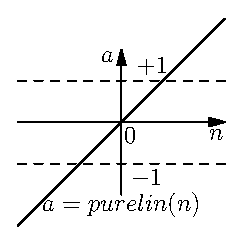
\includegraphics{octave/neuroPackage/graphics/purelin}
\caption{Linear transfer function}
\label{fig:purelinTransferFunction}
\end{figure}

\begin{figure}[htb]
\centering
  
\includegraphics{octave/neuroPackage/graphics/purelinlogo}
\caption{Linear transfer function logo}
\label{fig:purelinTransferFunctionLogo}
\end{figure}


\section{subset}
\subsection{subset}

\textit{subset} can be used to optimize the data sets for train, test and validation of a neural
network.\\

\noindent \textbf{\textcolor{brown}{Syntax:}}\\

\noindent [mTrain, mTest, mVali] = subset(mData,nTargets,iOpti,fTest,fVali);\\

\noindent \textbf{\textcolor{brown}{Description:}}\\

\noindent  \textbf{Left-Hand-Side:}\\
\noindent mTrain: (R+T) x M matrix with R input rows, T output rows and M columns
				where M <= N.\\
\noindent mTest:  (R+T) x S matrix with R input rows, T output rows and S columns
				where S <= N.\\
\noindent mVali:  (R+T) x U matrix with R input rows, T output rows and U columns
				where U <= N. And U can only exist, if S also exist.\\

\noindent  \textbf{Right-Hand-Side:}\\
\noindent mData: (R+T) x N matrix with R input rows, T output rows and N columns\\ 
\noindent nTargets: Number of T output rows\\ 
\noindent iOpti: Integer value to define level of optimization.\\
\noindent fTest: Fraction to define the percentage of data sets which should be used for testing. \\
\noindent fVali: Fraction to define the percentage of data sets which should be used for testing.\\

\noindent iOpti can have following values:\\
0	: no optimization\\
1	: will randomise the column order and rerange the columns containing min and max values to be in the train set\\
2	:	will NOT randomise the column order, but rerange the columns containing min and max values to be in the train set\\

\noindent fTest or fValie have following meaning:\\
Each of this arguments can be a fraction or zero. The value 1 is not allowed! The sum of both values
must also be smaller than 1!\\
Example: fTest = 1/3\\

\noindent \textbf{Default values}\\
\noindent iOpti		= 1\\
\noindent fTest		= 1/3\\
\noindent fVali		= 1/6\\

\noindent \textbf{\textcolor{brown}{Examples:}}\\

\noindent mTrain = subset(mData,2,1,0,0)\\
\noindent [mTrain,mTest] = subset(mData,2,1,1/3,0);\\
\noindent [mTrain,mTest,mVali] = subset(mData,1);\\
\noindent [mTrain,mTest,mVali] = subset(mData,1,1,1/3,1/6);\\
\section{\_\_analyzerows}
\begin{verbatim}
%!shared b, retmat
%! disp("testing __analyzerows")
%! b = [1 0 0 1; 1 0 0 0; 1 2 0 1];
%! retmat = __analyzerows(b);
%!assert(retmat(1,1)==1);#%!assert(retmat(1,1)==1);
%!assert(retmat(2,1)==1);
%!assert(retmat(3,1)==0);
%! b = [1 0 0 2; 1 0 0 0; 1 1 1 1];
%! retmat = __analyzerows(b);
%!assert(retmat(1,2)==0);
%!assert(retmat(2,2)==0);
%!assert(retmat(3,2)==1);
%! b = [1 0 0 2; 1 0 0 0; 1 1 1 1];
%! retmat = __analyzerows(b);
%!assert(retmat(1,3)==2);
%!assert(retmat(2,3)==0);
%!assert(retmat(3,3)==0);
%! retmat = __analyzerows(b);
%!assert(retmat(1,4)==1);
%!assert(retmat(2,4)==0);
%!assert(retmat(3,4)==0);
\end{verbatim}

\section{\_\_copycoltopos1}
\begin{verbatim}
%!shared a, retmat
%! disp("testing __copycoltopos1")
%! a = [0 1 2 3 4; 5 6 7 8 9];
%! retmat = __copycoltopos1(a,3);
%!assert(retmat(1,1)==2);
%!assert(retmat(2,1)==7);
%! retmat = __copycoltopos1(a,5);
%!assert(retmat(1,1)==4);
%!assert(retmat(2,1)==9);
\end{verbatim}

\section{\_\_optimizedatasets}
\begin{verbatim}
%!shared retmatrix, matrix
%! disp("testing __optimizedatasets")
%! matrix = [1 2 3 2 1 2 3 0 5 4 3 2 2 2 2 2 2; \
%!			 0 1 1 0 0 0 0 0 0 0 0 0 0 0 1 1 0; \
%!			-1 3 2 4 9 1 1 1 1 1 9 1 1 1 9 9 0; \
%!			 2 3 2 3 2 2 2 2 3 3 3 3 1 1 1 1 1];
%! ## The last row is equal to the neural network targets
%! retmatrix = __optimizedatasets(matrix,9,1);
%! ## the above statement can't be tested with assert!
%! ## it contains random values! So pass a "success" message
%!assert(1==1);
%! matrix = [1 2 3 2 1 2 3 0 5 4 3 2 2 2 2 2 2; \
%!			 0 1 1 0 0 0 0 0 0 0 0 0 0 0 1 1 0; \
%!			-1 3 2 4 9 1 1 1 1 1 9 1 1 1 9 9 0; \
%!			 2 3 2 3 2 2 2 2 3 3 3 3 1 1 1 1 1];
%! ## The last row is equal to the neural network targets
%! retmatrix = __optimizedatasets(matrix,9,1,0);
%!assert(retmatrix(1,1)==5);
%!assert(retmatrix(2,1)==0);
%!assert(retmatrix(3,1)==1);
%!assert(retmatrix(4,1)==3);
\end{verbatim}

\section{\_\_randomisecols}
\begin{verbatim}
%!# no test possible, contains randperm which is using
%!# some randome functions
\end{verbatim}

\section{\_\_rerangecolumns}
\begin{verbatim}
%!shared matrix,analyzeMatrix,nTrainSets, returnmatrix
%! disp("testing __rerangecolumns")
%! matrix = [0 1 0 0 0 0 1 0 1 1;  \
%!			 4 4 4 4 4 4 4 4 4 4;  \
%!        -1.1 -1.1 2 3 4 3.2 1 8 9 10; \
%!           0 1.1 3 4 5 2 10 10 2 3; \
%!          -1 1 1 1 1 2 3 4 1 5];
%! analyzeMatrix = [1 0 0 0; 0 1 0 0; 0 0 2 1; 0 0 1 2; 0 0 1 1];
%! nTrainSets = 8;
%! returnmatrix = __rerangecolumns(matrix,analyzeMatrix,nTrainSets);
%!assert(returnmatrix(1,1)==1);
%!assert(returnmatrix(2,1)==4);
%!assert(returnmatrix(3,1)==1);
%!assert(returnmatrix(4,1)==10);
%!assert(returnmatrix(5,1)==3);
%! matrix = [0 1 0 0 0 0 1 0 1 1; 			\
%!			 4 4 4 4 4 4 4 4 4 4; 			\
%!          -1.1 -1.1 2 3 4 3.2 1 8 9 10; 	\
%!           0 1.1 3 4 5 2 10 10 2 3; 		\
%!          -1 1 1 1 1 2 3 4 1 5;     		\
%!			 0 1 2 1 2 1 2 3 4 5;];  # the last row is euqal to the nnet targets
%! analyzeMatrix = [1 0 0 0; 0 1 0 0; 0 0 2 1; 0 0 1 2; 0 0 1 1];
%! nTrainSets = 8;
%! returnmatrix = __rerangecolumns(matrix,analyzeMatrix,nTrainSets);
%!assert(returnmatrix(1,1)==1);
%!assert(returnmatrix(2,1)==4);
%!assert(returnmatrix(3,1)==1);
%!assert(returnmatrix(4,1)==10);
%!assert(returnmatrix(5,1)==3);
%!assert(returnmatrix(6,1)==2);
\end{verbatim}


\chapter{analyzing matlab functions}

\section{analyzing newff}
First, \textit{newff} will be analyzed for a X-X-X mlp. This means, maximum 3 layers, including the input layer. Or in words, one input- one hidden- and one output-layer. The number of neurons are choosable.

Following command will be used, to create a new feed-forward neural network:\\
\noindent MLPnet = newff(mMinMaxElements,[nHiddenNeurons nOutputNeurons],...\newline
\{'tansig','purelin'\},'trainlm','learngdm','mse');\\

newff is the matlab command, mMinMaxElements is a $Rx2$-Matrix with minimum and maximum values of the inputs. $R$ is equal to the number of input neurons. [nHiddenNeurons nOutputNeurons] are the scalar values, to define the number of neurons in the hidden and output layer. One value, for each layer. \{'tansig','purelin'\} are the transfer functions, for each layer. This means, 'tansig' for the hidden layer and 'purelin' for the output layer. 'trainlm' is the training algorithm, in this case, Levenberg-Marquardt. 'learngdm' is the learn algorithm and 'mse' is the performance function, \textbf{m}ean-\textbf{s}quare-\textbf{e}rror.\\
MLPnet will be a structure with following content:

\begin{verbatim}
Neural Network object:

    architecture:

         numInputs: 1
         numLayers: 2
       biasConnect: [1; 1]
      inputConnect: [1; 0]
      layerConnect: [0 0; 1 0]
     outputConnect: [0 1]
     targetConnect: [0 1]

        numOutputs: 1  (read-only)
        numTargets: 1  (read-only)
    numInputDelays: 0  (read-only)
    numLayerDelays: 0  (read-only)

    subobject structures:

            inputs: {1x1 cell} of inputs
            layers: {2x1 cell} of layers
           outputs: {1x2 cell} containing 1 output
           targets: {1x2 cell} containing 1 target
            biases: {2x1 cell} containing 2 biases
      inputWeights: {2x1 cell} containing 1 input weight
      layerWeights: {2x2 cell} containing 1 layer weight

    functions:

          adaptFcn: 'trains'
           initFcn: 'initlay'
        performFcn: 'mse'
          trainFcn: 'trainlm'

    parameters:

        adaptParam: .passes
         initParam: (none)
      performParam: (none)
        trainParam: .epochs, .goal, .max_fail, .mem_reduc, 
                    .min_grad, .mu, .mu_dec, .mu_inc, 
                    .mu_max, .show, .time

    weight and bias values:

                IW: {2x1 cell} containing 1 input weight matrix
                LW: {2x2 cell} containing 1 layer weight matrix
                 b: {2x1 cell} containing 2 bias vectors

    other:

          userdata: (user stuff)
\end{verbatim}
\textit{numInputs: 1}: one input layer\\
\noindent \textit{numLayers: 2}: one hidden and one output layer\\
\noindent \textit{biasConnect: [1; 1]}: unknown till now!!\\
\noindent \textit{inputConnect: [1; 0]}: unknown till now!!\\
\noindent \textit{layerConnect: [0 0; 1 0]}: unknown till now!!\\
\noindent \textit{outputConnect: [0 1]}: unknown till now!!\\
\noindent \textit{targetConnect: [0 1]}: unknown till now!!\\
\noindent \textit{numOutputs: 1  (read-only)}: unknown till now!!\\
\noindent \textit{numTargets: 1  (read-only)}: unknown till now!!\\
\noindent \textit{numInputDelays: 0  (read-only)}: unknown till now!!\\
\noindent \textit{numLayerDelays: 0  (read-only)}: unknown till now!!\\
\noindent \textit{inputs: {1x1 cell} of inputs}: input layer definition\\
Because we have defined only one input layer, you can see the detailed definition with
following command in the matlab prompt:\\
\begin{verbatim}
	MLPnet.inputs{1}

ans = 

       range: [26x2 double]
        size: 26
    userdata: [1x1 struct]
\end{verbatim}
range are the min. and max. values of the inputs. size is the number of input neurons and userdata are user specified inputs...!\\
\noindent \textit{layers: {2x1 cell} of layers}: hidden and output layer definition\\
The dimension of $2x1 cell$ is because we have one hidden and one output layer. So too see the details of the hidden layer definitions, we have to enter:
\begin{verbatim}
K>> MLPnet.layers{1}

ans = 

     dimensions: 2
    distanceFcn: ''
      distances: []
        initFcn: 'initnw'
    netInputFcn: 'netsum'
      positions: [0 1]
           size: 2
    topologyFcn: 'hextop'
    transferFcn: 'tansig'
       userdata: [1x1 struct]
\end{verbatim}
and for the output layer:
\begin{verbatim}
K>> MLPnet.layers{2}

ans = 

     dimensions: 1
    distanceFcn: ''
      distances: []
        initFcn: 'initnw'
    netInputFcn: 'netsum'
      positions: 0
           size: 1
    topologyFcn: 'hextop'
    transferFcn: 'purelin'
       userdata: [1x1 struct]
\end{verbatim}

\noindent \textit{outputs: {1x2 cell} containing 1 output}: output layer definitions\\
\begin{verbatim}
K>> MLPnet.outputs

ans = 

     []    [1x1 struct]
\end{verbatim}
How knows, why this is a $1x2 cell$? The next command will also show the detailed definition! Of course, realy simple.
\begin{verbatim}
K>> MLPnet.outputs{2}

ans = 

        size: 1
    userdata: [1x1 struct]
\end{verbatim} 

\noindent \textit{targets: {1x2 cell} containing 1 target}: unknow till now\\

\noindent \textit{biases: {2x1 cell} containing 2 biases}: detailed definitions, for the biases\\
\begin{verbatim}
K>> MLPnet.biases

ans = 

    [1x1 struct]
    [1x1 struct]

K>> MLPnet.biases{1}

ans = 

       initFcn: ''
         learn: 1
      learnFcn: 'learngdm'
    learnParam: [1x1 struct]
          size: 2
      userdata: [1x1 struct]

K>> MLPnet.biases{2}

ans = 

       initFcn: ''
         learn: 1
      learnFcn: 'learngdm'
    learnParam: [1x1 struct]
          size: 1
      userdata: [1x1 struct]
\end{verbatim}
      inputWeights: {2x1 cell} containing 1 input weight
      layerWeights: {2x2 cell} containing 1 layer weight


\paragraph{weight and bias values:}

\subparagraph{IW:}
\begin{verbatim}
K>> MLPnet.IW

ans = 

    [2x26 double]
               []
\end{verbatim}

\subparagraph{LW:}
\begin{verbatim}
K>> MLPnet.LW

ans = 

              []     []
    [1x2 double]     []
\end{verbatim}

\subparagraph{b:}
\begin{verbatim}
K>> MLPnet.b

ans = 

    [2x1 double]
    [   -0.3908]
\end{verbatim}


\paragraph{net.trainParam:}
Output for the Levenberg-Marquardt train algorithm.
\begin{verbatim}
K>> MLPnet.trainParam

ans = 

       epochs: 100
         goal: 0
     max_fail: 5
    mem_reduc: 1
     min_grad: 1.0000e-010
           mu: 0.0010
       mu_dec: 0.1000
       mu_inc: 10
       mu_max: 1.0000e+010
         show: 25
         time: Inf
\end{verbatim}
\input{analyzing/analyzingNewp}


\appendix
\chapter{Examples}




\section{Example 1}
You can find this example in the \textit{tests/MLP} directory of each release or from the subversion repository. I will do (more or less) a line by line walkthrough, so after this should be everything clear. I assume that you have some experience with multilayer perceptrons.

\subsection{Introduction}
Our problem can be solved with a monotonically increasing or decreasing surface. An input vector \textbf{p} (with 9 values) should be mapped onto one output value. Because we know that it can be solved with a monotonically increasing or decreasing surface, we can choose a 9-1-1 multi-layer perceptron (short: MLP).
This means an MLP with 9 input neurons, only 1 hidden neuron and with 1 output neuron.

\subsection{Code m-file}
\noindent
\ttfamily
\hlstd{}\hlline{00001\ }\hlslc{\#\# Copyright (C) 2006 Michel D. Schmid}\hlstd{\ \ }\hlslc{$<$michaelschmid@users.sourceforge.net$>$}\\
\hlline{00002\ }\hlstd{}\hlslc{\#\#}\\
\hlline{00003\ }\hlstd{}\hlslc{\#\#}\\
\hlline{00004\ }\hlstd{}\hlslc{\#\# This program is free software; you can redistribute it and/or modify it}\\
\hlline{00005\ }\hlstd{}\hlslc{\#\# under the terms of the GNU General Public License as published by}\\
\hlline{00006\ }\hlstd{}\hlslc{\#\# the Free Software Foundation; either version 2, or (at your option)}\\
\hlline{00007\ }\hlstd{}\hlslc{\#\# any later version.}\\
\hlline{00008\ }\hlstd{}\hlslc{\#\#}\\
\hlline{00009\ }\hlstd{}\hlslc{\#\# This program is distributed in the hope that it will be useful, but}\\
\hlline{00010\ }\hlstd{}\hlslc{\#\# WITHOUT ANY WARRANTY; without even the implied warranty of}\\
\hlline{00011\ }\hlstd{}\hlslc{\#\# MERCHANTABILITY or FITNESS FOR A PARTICULAR PURPOSE.}\hlstd{\ \ }\hlslc{See the GNU}\\
\hlline{00012\ }\hlstd{}\hlslc{\#\# General Public License for more details.}\\
\hlline{00013\ }\hlstd{}\hlslc{\#\#}\\
\hlline{00014\ }\hlstd{}\hlslc{\#\# You should have received a copy of the GNU General Public License}\\
\hlline{00015\ }\hlstd{}\hlslc{\#\# along with this program; see the file COPYING.}\hlstd{\ \ }\hlslc{If not, write to the Free}\\
\hlline{00016\ }\hlstd{}\hlslc{\#\# Software Foundation, Inc., 51 Franklin Street, Fifth Floor, Boston, MA}\\
\hlline{00017\ }\hlstd{}\hlslc{\#\# 02110{-}1301, USA.}\\
\hlline{00018\ }\hlstd{}\\
\hlline{00019\ }\hlslc{\#\# Author: Michel D. Schmid}\\
\hlline{00020\ }\hlstd{}\\
\hlline{00021\ }\\
\hlline{00022\ }\hlslc{\#\# load data}\\
\hlline{00023\ }\hlstd{mData }\hlsym{= }\hlstd{}\hlkwc{load}\hlstd{}\hlsym{(}\hlstd{}\hlstr{"mData.txt"}\hlstd{}\hlsym{,}\hlstd{}\hlstr{"mData"}\hlstd{}\hlsym{);}\\
\hlline{00024\ }\hlstd{mData }\hlsym{= }\hlstd{mData.mData}\hlsym{;}\\
\hlline{00025\ }\hlstd{}\hlsym{{[}}\hlstd{nRows}\hlsym{, }\hlstd{nColumns}\hlsym{{]} = }\hlstd{}\hlkwc{size}\hlstd{}\hlsym{(}\hlstd{mData}\hlsym{);}\\
\hlline{00026\ }\hlstd{}\hlstd{\ \ \ \ }\hlstd{}\hlslc{\# this file contains 13 columns.}\\
\hlline{00027\ }\hlstd{}\hlstd{\ \ \ \ }\hlstd{}\hlslc{\# The first 12 columns are the inputs}\\
\hlline{00028\ }\hlstd{}\hlstd{\ \ \ \ }\hlstd{}\hlslc{\# the last column is the output,}\\
\hlline{00029\ }\hlstd{}\hlstd{\ \ \ \ }\hlstd{}\hlslc{\# remove column 4, 8 and 12!}\\
\hlline{00030\ }\hlstd{}\hlstd{\ \ \ \ }\hlstd{}\hlslc{\# 89 rows.}\\
\hlline{00031\ }\hlstd{\\
\hlline{00032\ }\\
\hlline{00033\ }mOutput }\hlsym{= }\hlstd{}\hlstd{mData}\hlstd{}\hlsym{(:,}\hlstd{}\hlkwa{end}\hlstd{}\hlsym{);}\\
\hlline{00034\ }\hlstd{mInput }\hlsym{= }\hlstd{}\hlstd{mData}\hlstd{}\hlsym{(:,}\hlstd{}\hlnum{1}\hlstd{}\hlsym{:}\hlstd{}\hlkwa{end}\hlstd{}\hlsym{{-}}\hlstd{}\hlnum{1}\hlstd{}\hlsym{);}\\
\hlline{00035\ }\hlstd{}\hlstd{mInput}\hlstd{}\hlsym{(:,{[}}\hlstd{}\hlnum{4 8 12}\hlstd{}\hlsym{{]}) = {[}{]}; }\hlstd{}\hlslc{\# delete column 4, 8 and 12}\\
\hlline{00036\ }\hlstd{}\\
\hlline{00037\ }\hlslc{\#\# now prepare data}\\
\hlline{00038\ }\hlstd{mInput }\hlsym{= }\hlstd{mInput}\hlstd{';}\\
\hlline{00039\ }\hlstd{mOutput = mOutput'}\hlstd{}\hlsym{;}\\
\hlline{00040\ }\hlstd{}\\
\hlline{00041\ }\hlslc{\# now split the data matrix in 3 pieces, train data, test data and validate data}\\
\hlline{00042\ }\hlstd{}\hlslc{\# the proportion should be about 1/2 train, 1/3 test and 1/6 validate data}\\
\hlline{00043\ }\hlstd{}\hlslc{\# in this neural network we have 12 weights, for each weight at least 3 train sets..}\\
\hlline{00044\ }\hlstd{}\hlslc{\# (that's a rule of thumb like 1/2, 1/3 and 1/6)}\\
\hlline{00045\ }\hlstd{}\hlslc{\# 1/2 of 89 = 44.5; let's take 44 for training}\\
\hlline{00046\ }\hlstd{nTrainSets }\hlsym{= }\hlstd{}\hlkwc{floor}\hlstd{}\hlsym{(}\hlstd{nRows}\hlsym{/}\hlstd{}\hlnum{2}\hlstd{}\hlsym{);}\\
\hlline{00047\ }\hlstd{}\hlslc{\# now the rest of the sets are again 100\%}\\
\hlline{00048\ }\hlstd{}\hlslc{\# ==$>$ 2/3 for test sets and 1/3 for validate sets}\\
\hlline{00049\ }\hlstd{nTestSets }\hlsym{= (}\hlstd{nRows}\hlsym{{-}}\hlstd{nTrainSets}\hlsym{)/}\hlstd{}\hlnum{3}\hlstd{}\hlsym{{*}}\hlstd{}\hlnum{2}\hlstd{}\hlsym{;}\\
\hlline{00050\ }\hlstd{nValiSets }\hlsym{= }\hlstd{nRows}\hlsym{{-}}\hlstd{nTrainSets}\hlsym{{-}}\hlstd{nTestSets}\hlsym{;}\\
\hlline{00051\ }\hlstd{\\
\hlline{00052\ }mValiInput }\hlsym{= }\hlstd{}\hlstd{mInput}\hlstd{}\hlsym{(:,}\hlstd{}\hlnum{1}\hlstd{}\hlsym{:}\hlstd{nValiSets}\hlsym{);}\\
\hlline{00053\ }\hlstd{mValliOutput }\hlsym{= }\hlstd{}\hlstd{mOutput}\hlstd{}\hlsym{(:,}\hlstd{}\hlnum{1}\hlstd{}\hlsym{:}\hlstd{nValiSets}\hlsym{);}\\
\hlline{00054\ }\hlstd{}\hlstd{mInput}\hlstd{}\hlsym{(:,}\hlstd{}\hlnum{1}\hlstd{}\hlsym{:}\hlstd{nValiSets}\hlsym{) = {[}{]};}\\
\hlline{00055\ }\hlstd{}\hlstd{mOutput}\hlstd{}\hlsym{(:,}\hlstd{}\hlnum{1}\hlstd{}\hlsym{:}\hlstd{nValiSets}\hlsym{) = {[}{]};}\\
\hlline{00056\ }\hlstd{mTestInput }\hlsym{= }\hlstd{}\hlstd{mInput}\hlstd{}\hlsym{(:,}\hlstd{}\hlnum{1}\hlstd{}\hlsym{:}\hlstd{nTestSets}\hlsym{);}\\
\hlline{00057\ }\hlstd{mTestOutput }\hlsym{= }\hlstd{}\hlstd{mOutput}\hlstd{}\hlsym{(:,}\hlstd{}\hlnum{1}\hlstd{}\hlsym{:}\hlstd{nTestSets}\hlsym{);}\\
\hlline{00058\ }\hlstd{}\hlstd{mInput}\hlstd{}\hlsym{(:,}\hlstd{}\hlnum{1}\hlstd{}\hlsym{:}\hlstd{nTestSets}\hlsym{) = {[}{]};}\\
\hlline{00059\ }\hlstd{}\hlstd{mOutput}\hlstd{}\hlsym{(:,}\hlstd{}\hlnum{1}\hlstd{}\hlsym{:}\hlstd{nTestSets}\hlsym{) = {[}{]};}\\
\hlline{00060\ }\hlstd{mTrainInput }\hlsym{= }\hlstd{}\hlstd{mInput}\hlstd{}\hlsym{(:,}\hlstd{}\hlnum{1}\hlstd{}\hlsym{:}\hlstd{nTrainSets}\hlsym{);}\\
\hlline{00061\ }\hlstd{mTrainOutput }\hlsym{= }\hlstd{}\hlstd{mOutput}\hlstd{}\hlsym{(:,}\hlstd{}\hlnum{1}\hlstd{}\hlsym{:}\hlstd{nTrainSets}\hlsym{);}\\
\hlline{00062\ }\hlstd{}\\
\hlline{00063\ }\hlsym{{[}}\hlstd{mTrainInputN}\hlsym{,}\hlstd{cMeanInput}\hlsym{,}\hlstd{cStdInput}\hlsym{{]} = }\hlstd{}\hlkwc{prestd}\hlstd{}\hlsym{(}\hlstd{mTrainInput}\hlsym{);}\hlstd{}\hlslc{\# standardize inputs}\\
\hlline{00064\ }\hlstd{}\\
\hlline{00065\ }\hlslc{\#\# comments: there is no reason to standardize the outputs because we have only}\\
\hlline{00066\ }\hlstd{}\hlslc{\# one output ...}\\
\hlline{00067\ }\hlstd{}\\
\hlline{00068\ }\hlslc{\# define the max and min inputs for each row}\\
\hlline{00069\ }\hlstd{mMinMaxElements }\hlsym{= }\hlstd{}\hlkwc{min\textunderscore max}\hlstd{}\hlsym{(}\hlstd{mTrainInputN}\hlsym{); }\hlstd{}\hlslc{\# input matrix with (R x 2)...}\\
\hlline{00070\ }\hlstd{}\\
\hlline{00071\ }\hlslc{\#\# define network}\\
\hlline{00072\ }\hlstd{nHiddenNeurons }\hlsym{= }\hlstd{}\hlnum{1}\hlstd{}\hlsym{;}\\
\hlline{00073\ }\hlstd{nOutputNeurons }\hlsym{= }\hlstd{}\hlnum{1}\hlstd{}\hlsym{;}\\
\hlline{00074\ }\hlstd{\\
\hlline{00075\ }MLPnet }\hlsym{= }\hlstd{}\hlkwc{newff}\hlstd{}\hlsym{(}\hlstd{mMinMaxElements}\hlsym{,{[}}\hlstd{nHiddenNeurons nOutputNeurons}\hlsym{{]},}\hlstd{$\backslash$\\
\hlline{00076\ }}\hlstd{\ \ \ \ \ \ \ \ }\hlstd{}\hlsym{\{}\hlstd{}\hlstr{"tansig"}\hlstd{}\hlsym{,}\hlstd{}\hlstr{"purelin"}\hlstd{}\hlsym{\},}\hlstd{}\hlstr{"trainlm"}\hlstd{}\hlsym{,}\hlstd{}\hlstr{""}\hlstd{}\hlsym{,}\hlstd{}\hlstr{"mse"}\hlstd{}\hlsym{);}\\
\hlline{00077\ }\hlstd{}\hlslc{\#\# for test purpose, define weights by hand}\\
\hlline{00078\ }\hlstd{MLPnet.IW}\hlsym{\{}\hlstd{}\hlnum{1}\hlstd{}\hlsym{,}\hlstd{}\hlnum{1}\hlstd{}\hlsym{\}(:) = }\hlstd{}\hlnum{1.5}\hlstd{}\hlsym{;}\\
\hlline{00079\ }\hlstd{MLPnet.LW}\hlsym{\{}\hlstd{}\hlnum{2}\hlstd{}\hlsym{,}\hlstd{}\hlnum{1}\hlstd{}\hlsym{\}(:) = }\hlstd{}\hlnum{0.5}\hlstd{}\hlsym{;}\\
\hlline{00080\ }\hlstd{MLPnet.b}\hlsym{\{}\hlstd{}\hlnum{1}\hlstd{}\hlsym{,}\hlstd{}\hlnum{1}\hlstd{}\hlsym{\}(:) = }\hlstd{}\hlnum{1.5}\hlstd{}\hlsym{;}\\
\hlline{00081\ }\hlstd{MLPnet.b}\hlsym{\{}\hlstd{}\hlnum{2}\hlstd{}\hlsym{,}\hlstd{}\hlnum{1}\hlstd{}\hlsym{\}(:) = }\hlstd{}\hlnum{0.5}\hlstd{}\hlsym{;}\\
\hlline{00082\ }\hlstd{}\\
\hlline{00083\ }\hlkwc{saveMLPStruct}\hlstd{}\hlsym{(}\hlstd{MLPnet}\hlsym{,}\hlstd{}\hlstr{"MLP3test.txt"}\hlstd{}\hlsym{);}\\
\hlline{00084\ }\hlstd{}\\
\hlline{00085\ }\hlslc{\#\# define validation data new, for matlab compatibility}\\
\hlline{00086\ }\hlstd{VV.P }\hlsym{= }\hlstd{mValiInput}\hlsym{;}\\
\hlline{00087\ }\hlstd{VV.T }\hlsym{= }\hlstd{mValliOutput}\hlsym{;}\\
\hlline{00088\ }\hlstd{}\\
\hlline{00089\ }\hlslc{\#\# standardize also the validate data}\\
\hlline{00090\ }\hlstd{VV.P }\hlsym{= }\hlstd{}\hlkwc{trastd}\hlstd{}\hlsym{(}\hlstd{VV.P}\hlsym{,}\hlstd{cMeanInput}\hlsym{,}\hlstd{cStdInput}\hlsym{);}\\
\hlline{00091\ }\hlstd{}\\
\hlline{00092\ }\hlsym{{[}}\hlstd{net}\hlsym{{]} = }\hlstd{}\hlkwc{train}\hlstd{}\hlsym{(}\hlstd{MLPnet}\hlsym{,}\hlstd{mTrainInputN}\hlsym{,}\hlstd{mTrainOutput}\hlsym{,{[}{]},{[}{]},}\hlstd{VV}\hlsym{);}\\
\hlline{00093\ }\hlstd{}\\
\hlline{00094\ }\hlslc{\# make preparations for net test and test MLPnet}\\
\hlline{00095\ }\hlstd{}\hlslc{\#}\hlstd{\ \ }\hlslc{standardise input \& output test data}\\
\hlline{00096\ }\hlstd{}\hlsym{{[}}\hlstd{mTestInputN}\hlsym{{]} = }\hlstd{}\hlkwc{trastd}\hlstd{}\hlsym{(}\hlstd{mTestInput}\hlsym{,}\hlstd{cMeanInput}\hlsym{,}\hlstd{cStdInput}\hlsym{);}\\
\hlline{00097\ }\hlstd{}\\
\hlline{00098\ }\hlsym{{[}}\hlstd{simOut}\hlsym{{]} = }\hlstd{}\hlkwc{sim}\hlstd{}\hlsym{(}\hlstd{net}\hlsym{,}\hlstd{mTestInputN}\hlsym{);}\\
\hlline{00099\ }\hlstd{simOut}\\
\mbox{}
\normalfont

\subsection{Walkthrough}
Till line number 0023 there is realy nothing interesting.\\
On line 0023 \& 0024 data will be loaded. This data matrix contains 13 columns. Column 4, 8 and 12 won't be used (this is because the datas are of a real world problem). Column 13 contains the target values.
So on the lines 0049 till 0051 this will be splittet into the corresponding peaces. A short repetition about the datas: Each line is a data set with 9 input values and one target value. On line 0038 and 0039 the datas are transposed. So we have now in each column one data set.\\

Now let's split the data matrix again in 3 pieces. The biggest part is for training the network. The second part for testing the trained network to be sure it's still possible to generalize with the net. And the third part, and the smallest one, for validate during training. This splitting happens on the lines 0041 till 0061.\\

Line 0063 is the first special command from this toolbox. This command will be used to pre-standardize the input datas. Do it ever! Non linear transfer functions will squash the whole input range to an small second range e.g. the transfer function \textit{tansig} will squash the datas between -1 and +1.\\

On line 0069 the next toolbox command will be used. This command \textit{min\_max} creates a $Rx2$ matrix of the complete input matrix. Don't ask me for what MATLAB(TM) this is using. I couldn't figure out it. One part is the number of input neurons, but for this, the range would not be needed. Who cares ;-)\\

Now it's time to create a structure which holds the informations about the neural network. The command \textbf{newff} can do it for us. See the complete line and actually, please use it only on this way, each other try will fail! This means, you can change the number of input neurons, the number of hidden neurons and the number of output neurons of course. But don't change the train algorithm or the performance function.\\

\textbf{saveMLPStruct} on line 0083 is a command which doesn't exist in MATLAB(TM). This will save the structure with the same informations you can see in MATLAB(TM) if you try to open the net-type.\\

The validation part on line 0086 \& 0087 is important. The naming convention is for MATLAB(TM) compatibility. For validate, you have to define a structure with the name \textbf{VV}. Inside this structure you have to define actually \textbf{VV.P} \& \textbf{VV.T} for validate inputs and validate targets. Bye the way, you have to pre-standardize them like the training input matrix. Use for this the command \textbf{trastd} like on line 0090.\\

\textbf{train} is the next toolbox command and of course one of the most important. Please also use this command like on line 0092. Nothing else will work.\\

The second last step is to standardize again datas. This time the test datas. See line 0096 for this and the last step. Simulate the network. This can be done with the command \textbf{sim}. This will be a critical part if someone else will write a toolbox with this command name!\\

I hope this short walkthrough will help for first steps. In next time, I will try to improve this documentation and of course, the toolbox commands. But time is realy rare.



\section{Example 2}
You can find this example in this directory but renamed to \textit{MLP9\_1\_1.m\_template}.
I will explain only differencies to the example1, so please read it first, if you haven't.

\subsection{Introduction}
Our problem can be solved with a monotonically increasing or decreasing surface. An input vector \textbf{p}
(with 9 values) should be mapped onto one output value.
Because we know that it can be solved with a monotonically increasing or decreasing surface,
we can choose a 9-1-1 multi-layer perceptron (short: MLP).
This means an MLP with 9 input neurons, only 1 hidden neuron and with 1 output neuron.

\subsection{Code m-file}
\noindent
\ttfamily
\hlstd{}\hlline{00001\ }\hlslc{\#\# Copyright (C) 2006 Michel D. Schmid}\hlstd{\ \ }\hlslc{$<$michaelschmid@users.sourceforge.net$>$}\\
\hlline{00002\ }\hlstd{}\hlslc{\#\#}\\
\hlline{00003\ }\hlstd{}\hlslc{\#\#}\\
\hlline{00004\ }\hlstd{}\hlslc{\#\# This program is free software; you can redistribute it and/or modify it}\\
\hlline{00005\ }\hlstd{}\hlslc{\#\# under the terms of the GNU General Public License as published by}\\
\hlline{00006\ }\hlstd{}\hlslc{\#\# the Free Software Foundation; either version 2, or (at your option)}\\
\hlline{00007\ }\hlstd{}\hlslc{\#\# any later version.}\\
\hlline{00008\ }\hlstd{}\hlslc{\#\#}\\
\hlline{00009\ }\hlstd{}\hlslc{\#\# This program is distributed in the hope that it will be useful, but}\\
\hlline{00010\ }\hlstd{}\hlslc{\#\# WITHOUT ANY WARRANTY; without even the implied warranty of}\\
\hlline{00011\ }\hlstd{}\hlslc{\#\# MERCHANTABILITY or FITNESS FOR A PARTICULAR PURPOSE.}\hlstd{\ \ }\hlslc{See the GNU}\\
\hlline{00012\ }\hlstd{}\hlslc{\#\# General Public License for more details.}\\
\hlline{00013\ }\hlstd{}\hlslc{\#\#}\\
\hlline{00014\ }\hlstd{}\hlslc{\#\# You should have received a copy of the GNU General Public License}\\
\hlline{00015\ }\hlstd{}\hlslc{\#\# along with this program; see the file COPYING.}\hlstd{\ \ }\hlslc{If not, write to the Free}\\
\hlline{00016\ }\hlstd{}\hlslc{\#\# Software Foundation, Inc., 51 Franklin Street, Fifth Floor, Boston, MA}\\
\hlline{00017\ }\hlstd{}\hlslc{\#\# 02110{-}1301, USA.}\\
\hlline{00018\ }\hlstd{}\\
\hlline{00019\ }\hlslc{\#\# Author: Michel D. Schmid}\\
\hlline{00020\ }\hlstd{}\\
\hlline{00021\ }\\
\hlline{00022\ }\hlslc{\#\# load data}\\
\hlline{00023\ }\hlstd{mData }\hlsym{= }\hlstd{}\hlkwc{load}\hlstd{}\hlsym{(}\hlstd{}\hlstr{"mData.txt"}\hlstd{}\hlsym{,}\hlstd{}\hlstr{"mData"}\hlstd{}\hlsym{);}\\
\hlline{00024\ }\hlstd{mData }\hlsym{= }\hlstd{mData.mData}\hlsym{;}\\
\hlline{00025\ }\hlstd{}\hlsym{{[}}\hlstd{nRows}\hlsym{, }\hlstd{nColumns}\hlsym{{]} = }\hlstd{}\hlkwc{size}\hlstd{}\hlsym{(}\hlstd{mData}\hlsym{);}\\
\hlline{00026\ }\hlstd{}\hlstd{\ \ \ \ }\hlstd{}\hlslc{\# this file contains 13 columns.}\\
\hlline{00027\ }\hlstd{}\hlstd{\ \ \ \ }\hlstd{}\hlslc{\# The first 12 columns are the inputs}\\
\hlline{00028\ }\hlstd{}\hlstd{\ \ \ \ }\hlstd{}\hlslc{\# the last column is the output,}\\
\hlline{00029\ }\hlstd{}\hlstd{\ \ \ \ }\hlstd{}\hlslc{\# remove column 4, 8 and 12!}\\
\hlline{00030\ }\hlstd{}\hlstd{\ \ \ \ }\hlstd{}\hlslc{\# 89 rows.}\\
\hlline{00031\ }\hlstd{\\
\hlline{00032\ }\\
\hlline{00033\ }mOutput }\hlsym{= }\hlstd{}\hlstd{mData}\hlstd{}\hlsym{(:,}\hlstd{}\hlkwa{end}\hlstd{}\hlsym{);}\\
\hlline{00034\ }\hlstd{mInput }\hlsym{= }\hlstd{}\hlstd{mData}\hlstd{}\hlsym{(:,}\hlstd{}\hlnum{1}\hlstd{}\hlsym{:}\hlstd{}\hlkwa{end}\hlstd{}\hlsym{{-}}\hlstd{}\hlnum{1}\hlstd{}\hlsym{);}\\
\hlline{00035\ }\hlstd{}\hlstd{mInput}\hlstd{}\hlsym{(:,{[}}\hlstd{}\hlnum{4 8 12}\hlstd{}\hlsym{{]}) = {[}{]}; }\hlstd{}\hlslc{\# delete column 4, 8 and 12}\\
\hlline{00036\ }\hlstd{}\\
\hlline{00037\ }\hlslc{\#\# now prepare data}\\
\hlline{00038\ }\hlstd{mInput }\hlsym{= }\hlstd{mInput}\hlstd{';}\\
\hlline{00039\ }\hlstd{mOutput = mOutput'}\hlstd{}\hlsym{;}\\
\hlline{00040\ }\hlstd{}\\
\hlline{00041\ }\hlslc{\# now split the data matrix in 3 pieces, train data, test data and validate data}\\
\hlline{00042\ }\hlstd{}\hlslc{\# the proportion should be about 1/2 train, 1/3 test and 1/6 validate data}\\
\hlline{00043\ }\hlstd{}\hlslc{\# in this neural network we have 12 weights, for each weight at least 3 train sets..}\\
\hlline{00044\ }\hlstd{}\hlslc{\# (that's a rule of thumb like 1/2, 1/3 and 1/6)}\\
\hlline{00045\ }\hlstd{}\hlslc{\# 1/2 of 89 = 44.5; let's take 44 for training}\\
\hlline{00046\ }\hlstd{nTrainSets }\hlsym{= }\hlstd{}\hlkwc{floor}\hlstd{}\hlsym{(}\hlstd{nRows}\hlsym{/}\hlstd{}\hlnum{2}\hlstd{}\hlsym{);}\\
\hlline{00047\ }\hlstd{}\hlslc{\# now the rest of the sets are again 100\%}\\
\hlline{00048\ }\hlstd{}\hlslc{\# ==$>$ 2/3 for test sets and 1/3 for validate sets}\\
\hlline{00049\ }\hlstd{nTestSets }\hlsym{= (}\hlstd{nRows}\hlsym{{-}}\hlstd{nTrainSets}\hlsym{)/}\hlstd{}\hlnum{3}\hlstd{}\hlsym{{*}}\hlstd{}\hlnum{2}\hlstd{}\hlsym{;}\\
\hlline{00050\ }\hlstd{nValiSets }\hlsym{= }\hlstd{nRows}\hlsym{{-}}\hlstd{nTrainSets}\hlsym{{-}}\hlstd{nTestSets}\hlsym{;}\\
\hlline{00051\ }\hlstd{\\
\hlline{00052\ }mValiInput }\hlsym{= }\hlstd{}\hlstd{mInput}\hlstd{}\hlsym{(:,}\hlstd{}\hlnum{1}\hlstd{}\hlsym{:}\hlstd{nValiSets}\hlsym{);}\\
\hlline{00053\ }\hlstd{mValliOutput }\hlsym{= }\hlstd{}\hlstd{mOutput}\hlstd{}\hlsym{(:,}\hlstd{}\hlnum{1}\hlstd{}\hlsym{:}\hlstd{nValiSets}\hlsym{);}\\
\hlline{00054\ }\hlstd{}\hlstd{mInput}\hlstd{}\hlsym{(:,}\hlstd{}\hlnum{1}\hlstd{}\hlsym{:}\hlstd{nValiSets}\hlsym{) = {[}{]};}\\
\hlline{00055\ }\hlstd{}\hlstd{mOutput}\hlstd{}\hlsym{(:,}\hlstd{}\hlnum{1}\hlstd{}\hlsym{:}\hlstd{nValiSets}\hlsym{) = {[}{]};}\\
\hlline{00056\ }\hlstd{mTestInput }\hlsym{= }\hlstd{}\hlstd{mInput}\hlstd{}\hlsym{(:,}\hlstd{}\hlnum{1}\hlstd{}\hlsym{:}\hlstd{nTestSets}\hlsym{);}\\
\hlline{00057\ }\hlstd{mTestOutput }\hlsym{= }\hlstd{}\hlstd{mOutput}\hlstd{}\hlsym{(:,}\hlstd{}\hlnum{1}\hlstd{}\hlsym{:}\hlstd{nTestSets}\hlsym{);}\\
\hlline{00058\ }\hlstd{}\hlstd{mInput}\hlstd{}\hlsym{(:,}\hlstd{}\hlnum{1}\hlstd{}\hlsym{:}\hlstd{nTestSets}\hlsym{) = {[}{]};}\\
\hlline{00059\ }\hlstd{}\hlstd{mOutput}\hlstd{}\hlsym{(:,}\hlstd{}\hlnum{1}\hlstd{}\hlsym{:}\hlstd{nTestSets}\hlsym{) = {[}{]};}\\
\hlline{00060\ }\hlstd{mTrainInput }\hlsym{= }\hlstd{}\hlstd{mInput}\hlstd{}\hlsym{(:,}\hlstd{}\hlnum{1}\hlstd{}\hlsym{:}\hlstd{nTrainSets}\hlsym{);}\\
\hlline{00061\ }\hlstd{mTrainOutput }\hlsym{= }\hlstd{}\hlstd{mOutput}\hlstd{}\hlsym{(:,}\hlstd{}\hlnum{1}\hlstd{}\hlsym{:}\hlstd{nTrainSets}\hlsym{);}\\
\hlline{00062\ }\hlstd{}\\
\hlline{00063\ }\hlsym{{[}}\hlstd{mTrainInputN}\hlsym{,}\hlstd{cMeanInput}\hlsym{,}\hlstd{cStdInput}\hlsym{{]} = }\hlstd{}\hlkwc{prestd}\hlstd{}\hlsym{(}\hlstd{mTrainInput}\hlsym{);}\hlstd{}\hlslc{\# standardize inputs}\\
\hlline{00064\ }\hlstd{}\\
\hlline{00065\ }\hlslc{\#\# comments: there is no reason to standardize the outputs because we have only}\\
\hlline{00066\ }\hlstd{}\hlslc{\# one output ...}\\
\hlline{00067\ }\hlstd{}\\
\hlline{00068\ }\hlslc{\# define the max and min inputs for each row}\\
\hlline{00069\ }\hlstd{mMinMaxElements }\hlsym{= }\hlstd{}\hlkwc{min\textunderscore max}\hlstd{}\hlsym{(}\hlstd{mTrainInputN}\hlsym{); }\hlstd{}\hlslc{\# input matrix with (R x 2)...}\\
\hlline{00070\ }\hlstd{}\\
\hlline{00071\ }\hlslc{\#\# define network}\\
\hlline{00072\ }\hlstd{nHiddenNeurons }\hlsym{= }\hlstd{}\hlnum{1}\hlstd{}\hlsym{;}\\
\hlline{00073\ }\hlstd{nOutputNeurons }\hlsym{= }\hlstd{}\hlnum{1}\hlstd{}\hlsym{;}\\
\hlline{00074\ }\hlstd{\\
\hlline{00075\ }MLPnet }\hlsym{= }\hlstd{}\hlkwc{newff}\hlstd{}\hlsym{(}\hlstd{mMinMaxElements}\hlsym{,{[}}\hlstd{nHiddenNeurons nOutputNeurons}\hlsym{{]},}\hlstd{$\backslash$\\
\hlline{00076\ }}\hlstd{\ \ \ \ \ \ \ \ }\hlstd{}\hlsym{\{}\hlstd{}\hlstr{"tansig"}\hlstd{}\hlsym{,}\hlstd{}\hlstr{"purelin"}\hlstd{}\hlsym{\},}\hlstd{}\hlstr{"trainlm"}\hlstd{}\hlsym{,}\hlstd{}\hlstr{""}\hlstd{}\hlsym{,}\hlstd{}\hlstr{"mse"}\hlstd{}\hlsym{);}\\
\hlline{00077\ }\hlstd{}\hlslc{\#\# for test purpose, define weights by hand}\\
\hlline{00078\ }\hlstd{MLPnet.IW}\hlsym{\{}\hlstd{}\hlnum{1}\hlstd{}\hlsym{,}\hlstd{}\hlnum{1}\hlstd{}\hlsym{\}(:) = }\hlstd{}\hlnum{1.5}\hlstd{}\hlsym{;}\\
\hlline{00079\ }\hlstd{MLPnet.LW}\hlsym{\{}\hlstd{}\hlnum{2}\hlstd{}\hlsym{,}\hlstd{}\hlnum{1}\hlstd{}\hlsym{\}(:) = }\hlstd{}\hlnum{0.5}\hlstd{}\hlsym{;}\\
\hlline{00080\ }\hlstd{MLPnet.b}\hlsym{\{}\hlstd{}\hlnum{1}\hlstd{}\hlsym{,}\hlstd{}\hlnum{1}\hlstd{}\hlsym{\}(:) = }\hlstd{}\hlnum{1.5}\hlstd{}\hlsym{;}\\
\hlline{00081\ }\hlstd{MLPnet.b}\hlsym{\{}\hlstd{}\hlnum{2}\hlstd{}\hlsym{,}\hlstd{}\hlnum{1}\hlstd{}\hlsym{\}(:) = }\hlstd{}\hlnum{0.5}\hlstd{}\hlsym{;}\\
\hlline{00082\ }\hlstd{}\\
\hlline{00083\ }\hlkwc{saveMLPStruct}\hlstd{}\hlsym{(}\hlstd{MLPnet}\hlsym{,}\hlstd{}\hlstr{"MLP3test.txt"}\hlstd{}\hlsym{);}\\
\hlline{00084\ }\hlstd{}\\
\hlline{00085\ }\hlslc{\#\# define validation data new, for matlab compatibility}\\
\hlline{00086\ }\hlstd{VV.P }\hlsym{= }\hlstd{mValiInput}\hlsym{;}\\
\hlline{00087\ }\hlstd{VV.T }\hlsym{= }\hlstd{mValliOutput}\hlsym{;}\\
\hlline{00088\ }\hlstd{}\\
\hlline{00089\ }\hlslc{\#\# standardize also the validate data}\\
\hlline{00090\ }\hlstd{VV.P }\hlsym{= }\hlstd{}\hlkwc{trastd}\hlstd{}\hlsym{(}\hlstd{VV.P}\hlsym{,}\hlstd{cMeanInput}\hlsym{,}\hlstd{cStdInput}\hlsym{);}\\
\hlline{00091\ }\hlstd{}\\
\hlline{00092\ }\hlsym{{[}}\hlstd{net}\hlsym{{]} = }\hlstd{}\hlkwc{train}\hlstd{}\hlsym{(}\hlstd{MLPnet}\hlsym{,}\hlstd{mTrainInputN}\hlsym{,}\hlstd{mTrainOutput}\hlsym{,{[}{]},{[}{]},}\hlstd{VV}\hlsym{);}\\
\hlline{00093\ }\hlstd{}\\
\hlline{00094\ }\hlslc{\# make preparations for net test and test MLPnet}\\
\hlline{00095\ }\hlstd{}\hlslc{\#}\hlstd{\ \ }\hlslc{standardise input \& output test data}\\
\hlline{00096\ }\hlstd{}\hlsym{{[}}\hlstd{mTestInputN}\hlsym{{]} = }\hlstd{}\hlkwc{trastd}\hlstd{}\hlsym{(}\hlstd{mTestInput}\hlsym{,}\hlstd{cMeanInput}\hlsym{,}\hlstd{cStdInput}\hlsym{);}\\
\hlline{00097\ }\hlstd{}\\
\hlline{00098\ }\hlsym{{[}}\hlstd{simOut}\hlsym{{]} = }\hlstd{}\hlkwc{sim}\hlstd{}\hlsym{(}\hlstd{net}\hlsym{,}\hlstd{mTestInputN}\hlsym{);}\\
\hlline{00099\ }\hlstd{simOut}\\
\mbox{}
\normalfont

\subsection{Walkthrough}
The difference to the example1 starts below the line number 0035.\\
The difference concerns only the pre-processing section where the data set is splittet into 
the three subsets. This time, the command \textbf{subset} is used, which makes the complete
example about 19 lines shorter!
On line 0023 \& 0024 data will be loaded. This data matrix contains 13 columns.
Column 4, 8 and 12 won't be used (this is because the datas are of a real world problem).
Column 13 contains the target values.\\

Now on line 35 we have to merge the input and output targets again. Subset will take the complete
matrix as argument! On line 42 happens the complete magic :-). Subset will return three 
subsets containing each time the input and output arguments. So this part must be splitet once more!
But this is very easy and happens at some specific positions below.\\

That's it, \textbf{subset} will help you to write short scripts!





% Preamble

%\documentclass[a4paper]{report}

%\usepackage[ngerman]{babel}
%\usepackage[T1]{fontenc}
%\usepackage[ansinew]{inputenc}


%%%%%%%%%%%%%%%%%%%%%%%%%%%%%%
% start text here!!

%\begin{document}

\begin{thebibliography}{XXXXXXX}

\bibitem [1]{1} John W. Eaton

GNU Octave Manual, Edition 3, PDF-Version, February 1997

\bibitem [2]{2} The MathWorks, Inc.

MATLAB Online-Help

\bibitem [3]{3} Steven W. Smith

The Scientist and Engineer's Guide to Digital Signal Processing
ISBN 0-9660176-3-3, California Technical Publishing, 1997

\bibitem [4]{4} Martin T. Hagan, Howard B. Demuth, Mark Beale

Neural Network Design, ISBN 0971732108, PWS Publishing Company, USA, Boston, 1996





\end{thebibliography}
%\end{document}



\end{document}


